\chapter{Neerslagvorming en oplosbaarheid}\label{ch:b1:precipitation}

Een druppel zilvernitraat valt in kraanwater en er verschijnt een witte
wolk: zilverchloride, gevormd uit de paar milligram chloride-ionen in
elke liter. Water dat door kalksteen sijpelt, voert calciumcarbonaat mee
en zet het weer af, een fractie van een millimeter per jaar, als de
stalactieten van een grot. Een niersteen is ook een neerslag. Elk van
deze verschijnselen is een evenwicht tussen een vaste stof en haar ionen
in oplossing, en één constante, het \omterm{def:b1:precipitation:solubility-product}{oplosbaarheidsproduct}, zegt of de
vaste stof ontstaat, hoeveel ervan oplost, en hoe haar \omterm{def:b1:precipitation:solubility}{oplosbaarheid}
verandert wanneer een ander ion of de pH verandert. Daarmee kan een
chemicus ionen van elkaar scheiden door ze na elkaar neer te slaan ---
de basis van de behandeling van mijnwater waarmee dit hoofdstuk eindigt.

\begin{recall}
Het schoolboek (jaar 6 en 12) mat de \omterm{def:b1:precipitation:solubility}{oplosbaarheid} in gram per liter en
identificeerde ionen aan de hand van de neerslagen die ze geven. De
evenwichtsconstante, het \omterm{def:b1:extent-q-and-k:quotient}{reactiequotiënt} $Q$ en de \omterm{def:b1:extent-q-and-k:activity}{activiteiten} (1 voor
een zuivere vaste stof of het oplosmiddel, $c/c^\circ$ voor een opgeloste
stof) werden opgesteld in
\cref{ch:b1:extent-q-and-k}: een reactie verloopt voorwaarts zolang
$Q < K$. De methode van de \omterm{def:b1:predominant-reaction:predominant-reaction}{predominante reactie} en de schaal van de
$\mathrm{p}K_a$-waarden komen uit
\cref{ch:b1:predominant-reaction}; $c^\circ = \qty{1}{mol/L}$ wordt niet
in de quotiënten geschreven.
\end{recall}

\begin{omfigure}
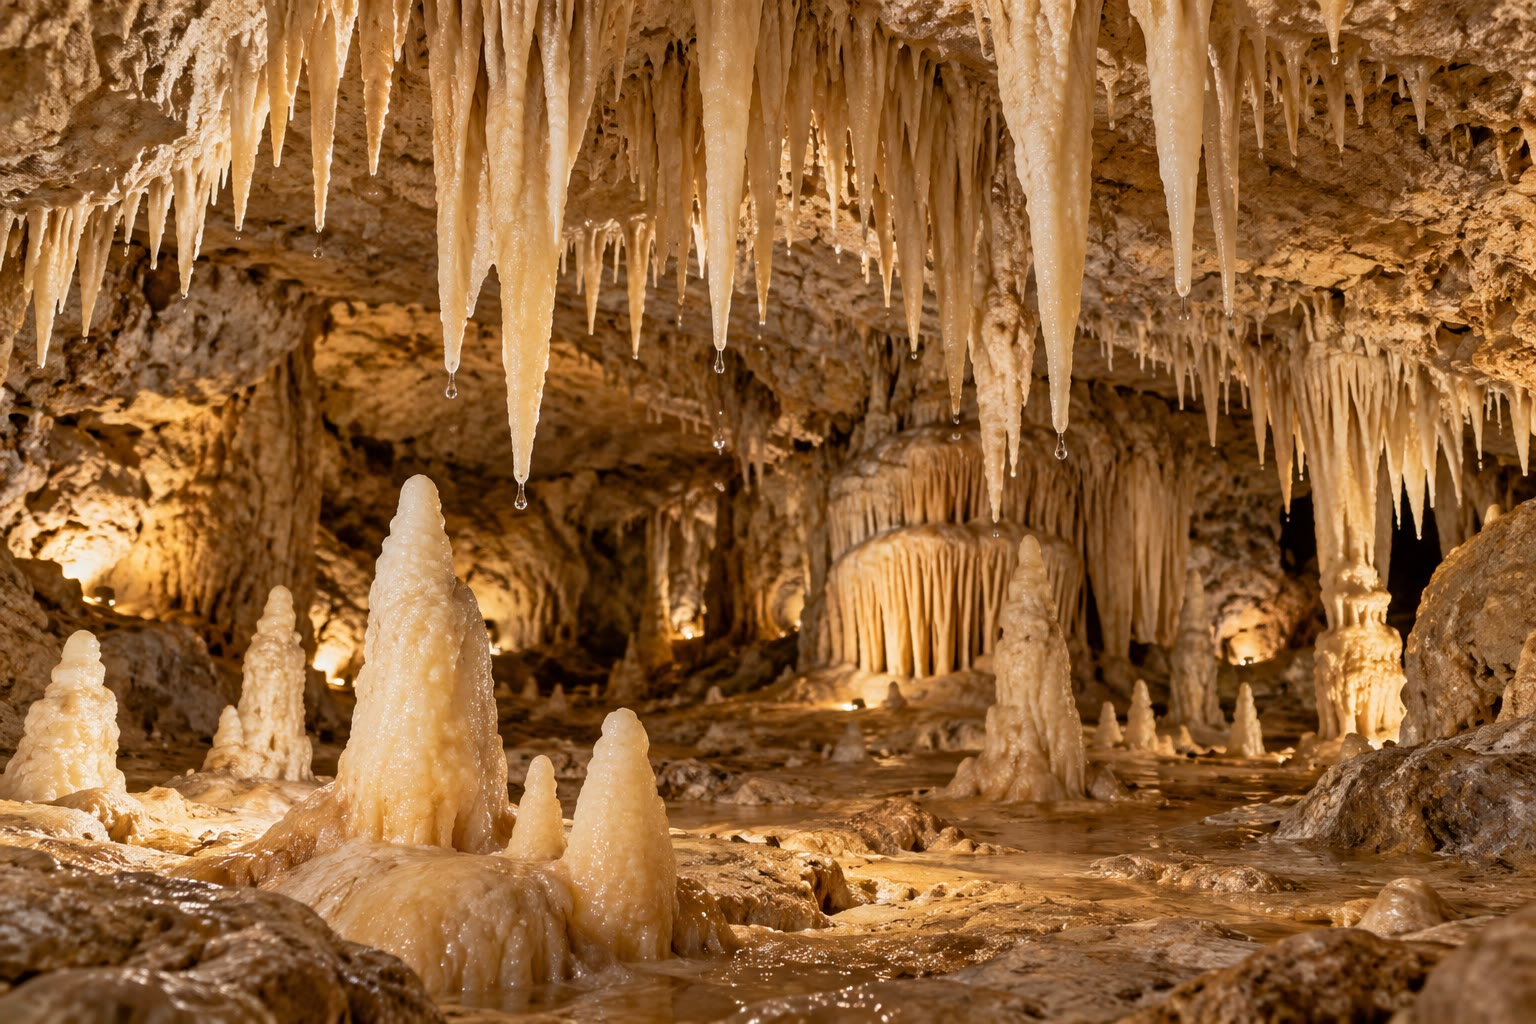
\includegraphics[width=0.62\linewidth]{images/book2/ai/b1-11-cave.jpg}

{\small Stalactieten en stalagmieten in een kalksteengrot. Water dat
rijk is aan koolstofdioxide lost in de bodem erboven calciumcarbonaat op;
in de grot verliest het een deel van zijn koolstofdioxide en slaat het
carbonaat opnieuw neer (\cref{exo:b1:precipitation:10}).}
\end{omfigure}

\section{Het oplosbaarheidsproduct}\label{sec:b1:precipitation:product}

Een \omterm{def:b1:crystals-metals:crystal}{kristal} zilverchloride dat in water valt, verliest ionen aan de
oplossing, en de oplossing geeft er een deel van terug aan het \omterm{def:b1:crystals-metals:crystal}{kristal}.
Wanneer de twee snelheden gelijk zijn, is de oplossing \emph{verzadigd}:
haar samenstelling verandert niet meer, hoewel er ionen in beide
richtingen blijven overgaan (figuur hieronder).

\begin{definition}[Oplosbaarheidsproduct]\label{def:b1:precipitation:solubility-product}
Het \emph{oplosbaarheidsproduct}\index{oplosbaarheidsproduct} $K_s$ van
een ionaire vaste stof $\mathrm{M}_a\mathrm{X}_b$ is de
evenwichtsconstante van haar oplossen in haar ionen,
\[
  \mathrm{M}_a\mathrm{X}_b\mathrm{(s)} \rightleftharpoons a\,\mathrm{M}^{m+}
  + b\,\mathrm{X}^{x-}, \qquad
  K_s = [\mathrm{M}^{m+}]_{\mathrm{eq}}^{\,a}\,[\mathrm{X}^{x-}]_{\mathrm{eq}}^{\,b},
  \qquad \mathrm{p}K_s = -\log K_s ,
\]
waarbij de \omterm{def:b1:extent-q-and-k:activity}{activiteit} van de vaste stof 1 is. Zoals elke
evenwichtsconstante hangt het alleen van de temperatuur af.
\end{definition}

Voor zilverchloride is \ce{AgCl(s) <=> Ag+ + Cl-} en $K_s =
[\ce{Ag+}][\ce{Cl-}] = 10^{-9.75}$; voor calciumfluoride \ce{CaF2(s) <=>
Ca^2+ + 2F-} en $K_s = [\ce{Ca^2+}][\ce{F-}]^2 = 10^{-9.84}$; voor
ijzer(III)hydroxide $K_s = [\ce{Fe^3+}][\ce{OH-}]^3 = 10^{-38.55}$.
De tabel hieronder geeft de waarden die in dit deel gebruikt worden.
Ze zijn, zoals de $\mathrm{p}K_a$-waarden van
\cref{ch:b1:predominant-reaction}, berekend uit getabelleerde
standaardvormingsenergieën van Gibbs: $\mathrm{p}K_s = \Delta_r G^\circ/(RT\ln 10)$,
een betrekking die in het deel van jaar~2 wordt afgeleid.

\begin{omfigure}
\begin{tikzpicture}[font=\small, >={Stealth}]
  % the crystal: alternating Ag+ (small, grey) and Cl- (large, green)
  \foreach \i in {0,1,2,3,4,5}
    \foreach \j in {0,1,2} {
      \pgfmathtruncatemacro{\pp}{mod(\i+\j,2)}
      \ifnum\pp=0
        \shade[ball color=green!55!black!60] (\i*0.62,\j*0.62) circle (0.29);
      \else
        \shade[ball color=gray!35] (\i*0.62,\j*0.62) circle (0.17);
      \fi }
  \draw[thick, gray] (-0.45,-0.45) rectangle (3.55,1.75);
  \node[below] at (1.55,-0.45) {\ce{AgCl(s)}};
  % ions in solution
  \shade[ball color=gray!35] (1.2,3.0) circle (0.17);
  \node[right] at (1.4,3.0) {\ce{Ag+}};
  \shade[ball color=green!55!black!60] (2.6,2.7) circle (0.29);
  \node[right] at (2.9,2.7) {\ce{Cl-}};
  \shade[ball color=gray!35] (4.4,1.4) circle (0.17);
  \shade[ball color=green!55!black!60] (5.1,2.6) circle (0.29);
  \shade[ball color=gray!35] (-1.0,2.4) circle (0.17);
  \shade[ball color=green!55!black!60] (-0.6,3.3) circle (0.29);
  % arrows: dissolution and precipitation
  \draw[->, thick, omDef] (1.24,1.6) to[bend left=20] node[left, pos=0.6] {oplossen} (1.15,2.78);
  \draw[->, thick, omProp] (2.55,2.38) to[bend left=20] node[right, pos=0.45] {neerslaan} (2.45,1.55);
  % the water line
  \draw[blue!50, thick] (-1.6,3.8) -- (5.9,3.8);
  \node[blue!60!black, anchor=east] at (5.9,4.05) {verzadigde oplossing};
\end{tikzpicture}

{\small Een \omterm{def:b1:crystals-metals:crystal}{kristal} zilverchloride in zijn verzadigde oplossing. Ionen
verlaten het oppervlak (oplossen) en andere worden ingevangen
(neerslaan), met dezelfde snelheid, zodat $[\ce{Ag+}][\ce{Cl-}]$ gelijk
blijft aan $K_s$. Zilverionen zijn kleiner getekend dan chloride-ionen,
zoals ze ook zijn.}
\end{omfigure}

\begin{omfigure}
\begin{tabular}{lc@{\qquad}lc}
\hline
vaste stof & $\mathrm{p}K_s$ & vaste stof & $\mathrm{p}K_s$ \\
\hline
\ce{AgCl} & 9.75 & \ce{Ca(OH)2} & 5.33 \\
\ce{AgBr} & 12.27 & \ce{Mg(OH)2} & 11.25 \\
\ce{AgI} & 16.07 & \ce{Fe(OH)2} & 16.31 \\
\ce{Ag2CrO4} & 11.95 & \ce{Zn(OH)2} & 16.38 \\
\ce{BaSO4} & 9.97 & \ce{Fe(OH)3} & 38.55 \\
\ce{CaCO3} (calciet) & 8.30 & \ce{Al(OH)3} (gibbsiet) & 34.75 \\
\ce{CaF2} & 9.84 & & \\
\hline
\end{tabular}

\smallskip
{\small \omterm{def:b1:precipitation:solubility-product}{Oplosbaarheidsproducten} bij \qty{25}{\celsius}, berekend uit de
standaardvormingsenergieën van Gibbs van de vaste stoffen en van de
ionen in water. Vormingsconstanten die in dit hoofdstuk gebruikt worden
(\cref{sec:b1:precipitation:amphoteric}):
$\log\beta_4 = 14.45$ voor \ce{Zn(OH)4^2-}, 33.52 voor \ce{Al(OH)4-}, en
$\log\beta_1 = 11.82$ voor \ce{FeOH^2+}.}
% ledger: dfg:AgCl_cr, dfg:AgBr_cr, dfg:AgI_cr, dfg:Ag2CrO4_cr, dfg:Ag+_ao, dfg:Cl-_ao, dfg:Br-_ao, dfg:I-_ao, dfg:CrO42-_ao (computed in figdata/bachelor-1/aqueous-constants.py)
% ledger: dfg:BaSO4_cr, dfg:Ba2+_ao, dfg:SO42-_ao, dfg:CaCO3_cr, dfg:CO32-_ao, dfg:CaF2_cr, dfg:Ca2+_ao, dfg:F-_ao (computed, same script)
% ledger: dfg:Ca_OH2_cr, dfg:Mg_OH2_cr, dfg:Mg2+_ao, dfg:Fe_OH2_cr, dfg:Fe2+_ao, dfg:Zn_OH2_cr, dfg:Zn2+_ao, dfg:Fe_OH3_cr, dfg:Fe3+_ao, dfg:Al2O3.3H2O_cr, dfg:Al3+_ao, dfg:OH-_ao (computed, same script)
% ledger: dfg:Zn_OH42-_ao, dfg:Al_OH4-_ao, dfg:FeOH2+_ao (formation constants, same script)
\end{omfigure}


\begin{proposition}[Voorwaarde voor neerslagvorming]\label{prop:b1:precipitation:precipitation-condition}
Een oplossing bevat de ionen van een vaste stof $\mathrm{M}_a\mathrm{X}_b$,
met \omterm{def:b1:extent-q-and-k:quotient}{reactiequotiënt} $Q_s = [\mathrm{M}^{m+}]^a[\mathrm{X}^{x-}]^b$ voor
het oplossen.
\begin{itemize}
  \item Als $Q_s < K_s$, kan de vaste stof bij evenwicht niet aanwezig
        zijn: de oplossing is onverzadigd en toegevoegde vaste stof lost
        op, volledig als het er niet te veel is.
  \item Als $Q_s > K_s$, slaat de vaste stof neer tot $Q_s = K_s$.
  \item De vaste stof en de oplossing bestaan alleen naast elkaar in
        evenwicht als $Q_s = K_s$.
\end{itemize}
\end{proposition}

\begin{proof}
Volgens \cref{ch:b1:extent-q-and-k} verloopt het oplossen voorwaarts
zolang $Q_s < K_s$ en achterwaarts (neerslagvorming) zolang $Q_s > K_s$.
Terwijl het oplossen voorwaarts verloopt, neemt $Q_s$ toe. Is de vaste
stof op voordat $Q_s$ de waarde $K_s$ bereikt, dan stopt de evolutie
zonder dat er vaste stof overblijft: een reactie met een zuivere
gecondenseerde \omterm{def:b1:extent-q-and-k:system}{fase} kan vóór het evenwicht stoppen, omdat de hoeveelheid
van die \omterm{def:b1:extent-q-and-k:system}{fase} niet negatief kan worden. Als $Q_s > K_s$, verlaagt de
neerslagvorming beide ionconcentraties en daalt $Q_s$ tot het gelijk is
aan $K_s$, wat altijd kan, omdat de ionen er zijn.
\end{proof}

Dat laatste punt onderscheidt een vaste stof van een opgelost deeltje.
Een zuur-basedeeltje is bij elke pH aanwezig, hoe weinig ook; een vaste
stof is aanwezig of afwezig. Daarom wordt haar diagram een
\emph{existentiediagram}, geen \omterm{def:b1:predominant-reaction:predominance}{predominantiediagram}
(\cref{sec:b1:precipitation:domains}).

\begin{example}[Twee oplossingen mengen]\label{ex:b1:precipitation:mixing}
\qty{10.0}{mL} zilvernitraat van \qty{2.0e-4}{mol/L} wordt gemengd met
\qty{10.0}{mL} natriumchloride van \qty{2.0e-4}{mol/L}. Net na het
mengen, vóór elke reactie, is $[\ce{Ag+}] = [\ce{Cl-}] = \qty{1.0e-4}{mol/L}$
en $Q_s = 10^{-8.0} > K_s = 10^{-9.75}$: zilverchloride slaat neer. Met
beide oplossingen op \qty{2.0e-6}{mol/L} is $Q_s = 10^{-12.0} < K_s$ en
blijft het mengsel helder. Zilvernitraat is een gevoelig reagens op
chloride-ionen, maar niet oneindig gevoelig.
\end{example}

\begin{inthelab}[De chloridetest]
In het practicumlokaal worden een paar druppels zilvernitraatoplossing
toegevoegd aan het monster, dat eerst met verdund salpeterzuur
aangezuurd is. Het zuur zet carbonaat- en hydroxide-ionen om in
koolstofdioxide en water; anders zouden ook die met zilverionen
neerslaan. Een wit neerslag dat in het licht donker wordt, is
zilverchloride; bromide geeft een roomkleurig neerslag en jodide een geel
(foto hieronder). Zilvernitraat kleurt de huid zwart: er worden
handschoenen en een veiligheidsbril gedragen.
\end{inthelab}

\begin{omfigure}
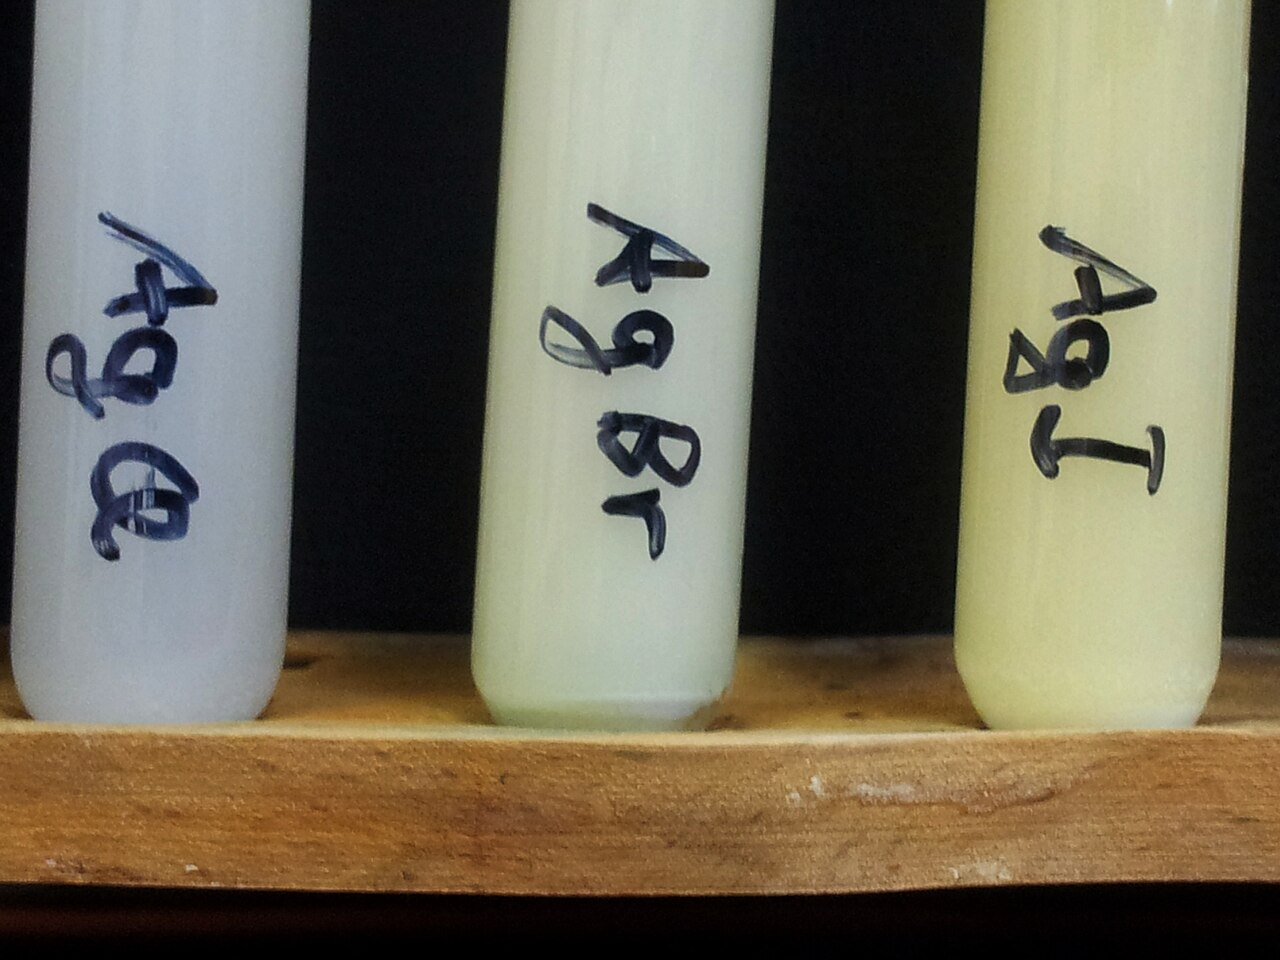
\includegraphics[width=0.6\linewidth]{images/book2/silver-halides.jpg}

{\small Neerslagen van zilverchloride (wit), zilverbromide (roomkleurig)
en zilverjodide (lichtgeel). Foto: Rrausch1974, CC BY-SA 3.0, Wikimedia
Commons.}
\end{omfigure}

\section{Oplosbaarheid}

\begin{definition}[Oplosbaarheid]\label{def:b1:precipitation:solubility}
De \emph{oplosbaarheid}\index{oplosbaarheid} $s$ van een vaste stof in
een gegeven oplossing is de hoeveelheid vaste stof die tot verzadiging
oplost in één liter van die oplossing (in \unit{mol/L}); vermenigvuldigd
met de molaire massa geeft ze de massaoplosbaarheid, in \unit{g/L}. Ze
hangt af van de temperatuur en van de samenstelling van de oplossing.
\end{definition}

\begin{proposition}[Oplosbaarheid uit het oplosbaarheidsproduct]\label{prop:b1:precipitation:s-of-ks}
In zuiver water, als de ionen aan geen enkele andere reactie deelnemen,
geldt
\[
  \mathrm{MX}:\ s = \sqrt{K_s}, \qquad
  \mathrm{MX_2}\ \text{of}\ \mathrm{M_2X}:\ s = \left(\frac{K_s}{4}\right)^{1/3},
  \qquad
  \mathrm{M}_a\mathrm{X}_b:\ s = \left(\frac{K_s}{a^a b^b}\right)^{1/(a+b)} .
\]
\end{proposition}

\begin{proof}
Als er per liter $s$ mol vaste stof oplost, is $[\mathrm{M}^{m+}] = as$ en
$[\mathrm{X}^{x-}] = bs$, dus bij verzadiging $K_s = (as)^a(bs)^b =
a^a b^b s^{a+b}$. Voor MX is $a = b = 1$; voor \ce{MX2} is $1^1 2^2 = 4$,
en hetzelfde voor \ce{M2X}.
\end{proof}

\begin{example}[Zilverchloride en zilverchromaat]\label{ex:b1:precipitation:agcl-ag2cro4}
Zilverchloride: $s = 10^{-9.75/2} = \qty{1.3e-5}{mol/L}$, of
\qty{1.9}{mg/L} met $M = \qty{143.4}{g/mol}$. Zilverchromaat \ce{Ag2CrO4}
($\mathrm{p}K_s = 11.95$): $s = (10^{-11.95}/4)^{1/3} =
\qty{6.6e-5}{mol/L}$. Het chromaat heeft de kleinere $K_s$ en is toch
vijf keer beter oplosbaar. \omterm{def:b1:precipitation:solubility-product}{Oplosbaarheidsproducten} kunnen alleen
rechtstreeks vergeleken worden tussen vaste stoffen met hetzelfde
formuletype.
\end{example}

\begin{remark}
De formules veronderstellen dat de ionen vrij zijn. In zuiver water is
het chromaation een \omterm{def:b1:predominant-reaction:strong-acid}{zwakke base} en wordt het zilverion door niets
gecomplexeerd, zodat het resultaat voor zilverchromaat vrijwel juist is;
voor een carbonaat, een sulfide of een hydroxide doen de base-eigenschappen
van het anion ertoe en is de volgende paragraaf nodig. Bij een hoge
ionsterkte wijken de \omterm{def:b1:extent-q-and-k:activity}{activiteiten} ook af van de concentraties, een
correctie die aan het deel van jaar~2 wordt overgelaten.
\end{remark}

\section{Effect van een gemeenschappelijk ion en van de pH}

\begin{definition}[Effect van een gemeenschappelijk ion]\label{def:b1:precipitation:common-ion}
Het \emph{effect van een gemeenschappelijk ion}\index{effect van een gemeenschappelijk ion}
is de daling van de \omterm{def:b1:precipitation:solubility}{oplosbaarheid} van een vaste stof in een oplossing die
al een van haar ionen bevat.
\end{definition}

\begin{proposition}[Oplosbaarheid met een gemeenschappelijk ion]\label{prop:b1:precipitation:common-ion}
MX lost op in een oplossing waarin al $[\mathrm{X}^-] = c$, met
$c \gg \sqrt{K_s}$. Dan is $s \approx K_s/c$, veel kleiner dan in zuiver
water. Voor \ce{MX2} in een oplossing die \ce{M^2+} op $c$ bevat, is
$s \approx \frac12\sqrt{K_s/c}$.
\end{proposition}

\begin{proof}
Bij verzadiging is $[\mathrm{M}^+] = s$ en $[\mathrm{X}^-] = c + s$, dus
$s(c + s) = K_s$. Als $s \ll c$, is $s = K_s/c$; de aanname klopt, omdat
$K_s/c \ll c$ wanneer $c^2 \gg K_s$. Voor \ce{MX2} is $[\ce{X-}] = 2s$ en
$[\mathrm{M}^{2+}] = c + s \approx c$, dus $c\,(2s)^2 = K_s$.
\end{proof}

Zilverchloride in natriumchloride van \qty{0.10}{mol/L}: $s = 10^{-9.75}/0.10
= \qty{1.8e-9}{mol/L}$, zevenduizend keer minder dan in water. Daarom
wordt een neerslag gewassen met een verdunde oplossing van een
gemeenschappelijk ion in plaats van met zuiver water: zo gaat er minder
van verloren.

Wanneer het anion van de vaste stof een base is, trekt een zuur het uit
het oplosevenwicht en stijgt de \omterm{def:b1:precipitation:solubility}{oplosbaarheid}. Voor calciumcarbonaat in
zuur geldt
\[
  \ce{CaCO3(s) + H3O+ <=> Ca^2+ + HCO3- + H2O}, \qquad
  K = \frac{K_s}{K_{a2}} = 10^{-8.30 + 10.33} = 10^{2.03} ,
\]
een begunstigde reactie: azijn of zoutzuur lost kalksteen op, en het
koolstofdioxide dat ontstaat door de verdere reactie van
\ce{HCO3-} geeft het bekende bruisen.
% ledger: dfg:HCO3-_ao (pKa2 of carbonic acid, ch. 10)


\begin{proposition}[Oplosbaarheid van een hydroxide als functie van de pH]\label{prop:b1:precipitation:hydroxide-ph}
In een oplossing die op een gegeven pH gebufferd is, gehoorzaamt de
concentratie van \ce{M^{n+}} in evenwicht met het hydroxide
\ce{M(OH)_n} aan
\[
  \log[\mathrm{M}^{n+}] = -\mathrm{p}K_s + n\,(\mathrm{p}K_e - \mathrm{pH}) ,
\]
een rechte met richtingscoëfficiënt $-n$ als functie van de pH. Als het
ion geen complex vormt, is dit de \omterm{def:b1:precipitation:solubility}{oplosbaarheid} van het hydroxide.
\end{proposition}

\begin{proof}
$K_s = [\mathrm{M}^{n+}][\ce{OH-}]^n$ en $[\ce{OH-}] = K_e/[\ce{H3O+}]$,
dus $\log[\mathrm{M}^{n+}] = \log K_s - n\log[\ce{OH-}] = -\mathrm{p}K_s -
n(\mathrm{pH} - \mathrm{p}K_e)$.
\end{proof}

Elke pH-eenheid deelt de \omterm{def:b1:precipitation:solubility}{oplosbaarheid} van ijzer(III)hydroxide door
duizend en die van zinkhydroxide door honderd. Hydroxiden worden
neergeslagen, en weer opgelost, door de pH te veranderen.

\begin{example}[Calciumcarbonaat oplossen met koolstofdioxide]\label{ex:b1:precipitation:cave}
Water dat opgelost koolstofdioxide bevat, lost calciet op:
\[
  \ce{CaCO3(s) + CO2(aq) + H2O <=> Ca^2+ + 2HCO3-}, \qquad
  K = \frac{K_s K_{a1}}{K_{a2}} = 10^{-8.30 - 6.37 + 10.33} = 10^{-4.34} ,
\]
waarbij de constante verkregen wordt door het oplossen van het carbonaat,
de eerste zuurfunctie van koolstofdioxide en de omgekeerde van de tweede
op te tellen. Hoe meer koolstofdioxide, hoe meer calciumcarbonaat er
oplost. Bodemlucht is meestal veel rijker aan koolstofdioxide dan de
lucht van een grot; water dat door de bodem gezakt is en het plafond van
de grot bereikt, verliest koolstofdioxide, en er zet zich calciet af
(\cref{exo:b1:precipitation:10}).
\end{example}

\section{Existentiegebieden en selectieve neerslagvorming}\label{sec:b1:precipitation:domains}

\begin{definition}[Existentiegebied]\label{def:b1:precipitation:existence-domain}
Voor een vaste stof en een gegeven totale concentratie $c$ van een van
haar ionen is het \emph{existentiegebied}\index{existentiegebied} van de
vaste stof het bereik van de variabele (pX, pM of pH) waarover de vaste
stof bij evenwicht aanwezig is. De grens ervan is de waarde waarbij het
eerste korreltje vaste stof verschijnt, wanneer $Q_s = K_s$ terwijl het
ion nog steeds op concentratie $c$ is.
\end{definition}

\begin{method}[Een existentiediagram tekenen]\label{met:b1:precipitation:existence-domain}
\begin{enumerate}
  \item Leg de totale concentratie $c$ vast van het ion dat niet op de as
        staat (bijvoorbeeld $[\ce{Ag+}]_{\mathrm{tot}} = c$ op een
        pCl-as).
  \item Schrijf $K_s$ op bij het begin van de neerslagvorming, met dat ion
        nog op $c$, en los op naar de variabele op de as.
  \item De vaste stof bestaat aan de kant waar het andere ion
        geconcentreerd is: kleine pCl (veel chloride), kleine pAg, of
        hoge pH voor een hydroxide.
  \item Duid geen gebied aan voor het ion zelf: het is overal aanwezig,
        op $c$ buiten het gebied van de vaste stof en onder $c$ erbinnen.
\end{enumerate}
\end{method}

Voor zilverchloride met $c = [\ce{Ag+}]_{\mathrm{tot}} = 10^{-2}$ begint
de neerslagvorming wanneer $[\ce{Cl-}] = K_s/c = 10^{-7.75}$, zodat de
vaste stof bestaat voor $\mathrm{pCl} < 7.75$. Voor zilverjodide ligt de
grens bij $\mathrm{pI} = 16.07 - 2 = 14.07$, zoals hieronder getekend.

\begin{omfigure}
\begin{tikzpicture}[font=\small, >={Stealth}, x=0.62cm]
  \fill[omDef!18] (0,0.12) rectangle (7.75,0.6);
  \draw[->, thick] (0,0) -- (17.2,0) node[right] {pCl of pI};
  \foreach \x in {0,2,4,6,8,10,12,14,16}
    \draw (\x,0.08) -- (\x,-0.08) node[below] {\x};
  \draw[omDef, thick] (7.75,-0.5) -- (7.75,0.9);
  \node[omDef] at (3.9,0.36) {\ce{AgCl(s)} bestaat};
  \node[omDef, above] at (7.75,0.9) {7.75};
  \node[anchor=west] at (8.0,0.36) {geen vaste stof: \ce{Ag+} op $10^{-2}$ mol/L};
  % AgI below
  \begin{scope}[yshift=-1.9cm]
  \fill[omProp!20] (0,0.12) rectangle (14.07,0.6);
  \draw[->, thick] (0,0) -- (17.2,0);
  \foreach \x in {0,2,4,6,8,10,12,14,16}
    \draw (\x,0.08) -- (\x,-0.08) node[below] {\x};
  \draw[omProp, thick] (14.07,-0.5) -- (14.07,0.9);
  \node[omProp] at (7.0,0.36) {\ce{AgI(s)} bestaat};
  \node[omProp, above] at (14.07,0.9) {14.07};
  \end{scope}
\end{tikzpicture}

{\small \omterm{def:b1:precipitation:existence-domain}{Existentiegebieden} van zilverchloride (op een pCl-as, boven) en
zilverjodide (op een pI-as, onder) voor een totale zilverconcentratie
van \qty{1.0e-2}{mol/L}. Jodide slaat zilver neer bij concentraties die
een miljoen keer lager zijn dan bij chloride.}
\end{omfigure}

\begin{method}[Selectieve neerslagvorming]\label{met:b1:precipitation:selective}
Zo scheid je twee ionen die met hetzelfde reagens neerslaan:
\begin{enumerate}
  \item bereken voor elk ion, bij zijn concentratie, de
        reagensconcentratie (of de pH) waarbij zijn vaste stof begint te
        ontstaan; het ion met de laagste waarde slaat eerst neer;
  \item bereken de concentratie van het eerste ion die in oplossing
        overblijft wanneer het tweede begint neer te slaan;
  \item de scheiding is aanvaardbaar als die concentratie een voldoende
        kleine fractie van de beginconcentratie is --- typisch
        \qty{0.1}{\percent} --- en de toevoeging van het reagens wordt dan
        tussen de twee drempels gestopt.
\end{enumerate}
\end{method}

\begin{example}[Jodide en chloride]\label{ex:b1:precipitation:i-cl}
Een oplossing bevat jodide- en chloride-ionen, beide op
\qty{1.0e-2}{mol/L}; er wordt druppelsgewijs zilvernitraat toegevoegd,
zonder verdunning. Zilverjodide begint te ontstaan bij $[\ce{Ag+}] = 10^{-16.07 + 2} =
10^{-14.07}$, zilverchloride bij $10^{-9.75 + 2} = 10^{-7.75}$: jodide
slaat eerst neer. Wanneer zilverchloride verschijnt, is
$[\ce{I-}] = 10^{-16.07}/10^{-7.75} = 10^{-8.32} = \qty{4.8e-9}{mol/L}$,
een fractie $5 \times 10^{-7}$ van het jodide: de scheiding is volledig.
\end{example}

Hydroxiden worden op dezelfde manier gescheiden, met de pH als
variabele. De grafiek hieronder toont, voor zes ionen op
\qty{0.010}{mol/L}, de pH waarbij het hydroxide verschijnt en de pH
waarbij \qty{99.9}{\percent} van het ion neergeslagen is. IJzer(III) en
aluminium worden in zuur water verwijderd, zink en ijzer(II) rond de
neutraliteit, magnesium rond pH 10 en calcium pas in zeer basisch
water.

\begin{omfigure}
\begin{tikzpicture}
\begin{axis}[
  width=0.82\linewidth, height=5.4cm, xmin=0, xmax=14, ymin=0.4, ymax=6.6,
  axis x line=bottom, axis y line=left, xlabel={pH},
  xtick={0,2,4,6,8,10,12,14}, ytick={1,2,3,4,5,6},
  yticklabels={\ce{Fe^3+}, \ce{Al^3+}, \ce{Zn^2+}, \ce{Fe^2+}, \ce{Mg^2+}, \ce{Ca^2+}},
  y dir=reverse, axis line style={-},
  tick label style={font=\small}, label style={font=\small}]
\addplot[draw=none, omDef!35,
  error bars/.cd, x dir=plus, x explicit,
  error bar style={line width=7pt, omDef!35}, error mark=none]
  table[x=start, y=row, x error expr=14-\thisrow{start}] {figdata/out/bachelor-1-solubility-ph-thresholds.dat};
\addplot[draw=none, omDef,
  error bars/.cd, x dir=plus, x explicit,
  error bar style={line width=7pt, omDef}, error mark=none]
  table[x=start, y=row, x error expr=\thisrow{end}-\thisrow{start}] {figdata/out/bachelor-1-solubility-ph-thresholds.dat};
\end{axis}
\end{tikzpicture}

{\small Neerslagvorming van hydroxiden uit oplossingen met
\qty{0.010}{mol/L} van elk ion. De donkere balk loopt van het eerste
korreltje hydroxide tot de pH waarbij \qty{99.9}{\percent} van het ion
neergeslagen is (één pH-eenheid breed voor een driewaardig ion, anderhalf
voor een tweewaardig); de lichte balk is de rest van het
\omterm{def:b1:precipitation:existence-domain}{existentiegebied} van het hydroxide. Het amfotere heroplossen van zink-
en aluminiumhydroxide bij hoge pH
(\cref{sec:b1:precipitation:amphoteric}) is niet weergegeven.}
\end{omfigure}

\section{Amfotere hydroxiden}\label{sec:b1:precipitation:amphoteric}

Voeg druppelsgewijs natronloog toe aan een oplossing van zinksulfaat: er
ontstaat een wit neerslag van zinkhydroxide, dat bij een overmaat
hydroxide weer oplost. Aluminiumhydroxide doet hetzelfde;
ijzer(III)hydroxide en magnesiumhydroxide niet.

\begin{definition}[Amfoteer hydroxide]\label{def:b1:precipitation:amphoteric-hydroxide}
Een hydroxide is een \emph{amfoteer hydroxide}\index{amfoteer hydroxide}
als het zowel in zuur oplost, als het kation, als in een overmaat base,
als een anionisch hydroxocomplex:
\[
  \ce{Zn(OH)2(s) + 2H3O+ -> Zn^2+ + 4H2O}, \qquad
  \ce{Zn(OH)2(s) + 2OH- -> Zn(OH)4^2-} .
\]
\end{definition}

Het complexe anion \ce{Zn(OH)4^2-} (tetrahydroxozincaat) wordt
gekenmerkt door zijn vormingsconstante
$\beta_4 = [\ce{Zn(OH)4^2-}]/([\ce{Zn^2+}][\ce{OH-}]^4)
= 10^{14.45}$; complexen en hun constanten zijn het onderwerp van
\cref{ch:b1:complexation}.

\begin{proposition}[Oplosbaarheid van een amfoteer hydroxide]\label{prop:b1:precipitation:amphoteric}
Als zink in oplossing alleen als \ce{Zn^2+} en \ce{Zn(OH)4^2-} voorkomt,
is de \omterm{def:b1:precipitation:solubility}{oplosbaarheid} van zinkhydroxide
\[
  s = [\ce{Zn^2+}] + [\ce{Zn(OH)4^2-}] = \frac{K_s}{[\ce{OH-}]^2} + K\,[\ce{OH-}]^2,
  \qquad K = \beta_4 K_s = 10^{-1.93} .
\]
In een grafiek van $\log s$ tegen de pH volgt ze een rechte met
richtingscoëfficiënt $-2$ bij lage pH en een rechte met
richtingscoëfficiënt $+2$ bij hoge pH. Ze is het kleinst bij
$[\ce{OH-}]^4 = K_s/K = 1/\beta_4$, dus bij $\mathrm{pH} =
\mathrm{p}K_e - \frac14\log\beta_4$, waar $s_{\min} = 2\sqrt{K_s K}$.
\end{proposition}

\begin{proof}
Bij verzadiging is $[\ce{Zn^2+}] = K_s/[\ce{OH-}]^2$, en
$[\ce{Zn(OH)4^2-}] = \beta_4[\ce{Zn^2+}][\ce{OH-}]^4 = \beta_4 K_s
[\ce{OH-}]^2$. Met $w = [\ce{OH-}]^2$ heeft $s(w) = K_s/w + Kw$ de
afgeleide $-K_s/w^2 + K$, die nul is bij $w = \sqrt{K_s/K}$, waar
$s = 2\sqrt{K_s K}$. Bij lage pH overheerst de eerste term en is
$\log s = \log K_s - 2\log[\ce{OH-}]$ (richtingscoëfficiënt $-2$ in de
pH); bij hoge pH de tweede, $\log s = \log K + 2\log[\ce{OH-}]$
(richtingscoëfficiënt $+2$).
\end{proof}

Met de waarden hierboven ligt het minimum bij $\mathrm{pH} = 14.00 - 14.45/4
= 10.39$ en is $s_{\min} = 2 \times 10^{-(16.38 + 1.93)/2} =
\qty{1.4e-9}{mol/L}$
(figuur hieronder). Het echte minimum ligt veel hoger: zink vormt ook
\ce{ZnOH+}, \ce{Zn(OH)3-} en vooral een ongeladen opgelost
\ce{Zn(OH)2(aq)}, waarvan de concentratie in evenwicht met de vaste stof
niet van de pH afhangt. De volledige berekening, met dezelfde tabellen,
legt de bodem rond
$10^{-5.6}$~mol/L. Een model met twee deeltjes geeft de
richtingscoëfficiënten en de volgorde van de drempels; rond het minimum
telt elk deeltje mee.

\begin{omfigure}
\begin{tikzpicture}
\begin{axis}[name=zn,
  width=0.46\linewidth, height=5.6cm, xmin=6, xmax=14, ymin=-10, ymax=0,
  axis x line=bottom, axis y line=left, xlabel={pH}, ylabel={$\log s$},
  xtick={6,8,10,12,14}, ytick={-10,-8,-6,-4,-2,0},
  tick label style={font=\small}, label style={font=\small}]
\addplot[omProp, dashed, thick] table[x=pH, y=full] {figdata/out/bachelor-1-solubility-ph-zinc.dat};
\addplot[omDef, very thick] table[x=pH, y=model] {figdata/out/bachelor-1-solubility-ph-zinc.dat};
\node[font=\small, anchor=west] at (axis cs:7.0,-1.0) {\ce{Zn^2+}};
\node[font=\small, anchor=east] at (axis cs:13.8,-1.1) {\ce{Zn(OH)4^2-}};
\node[font=\small, omProp, anchor=south] at (axis cs:10.4,-5.5) {alle deeltjes};
\node[font=\small, anchor=north] at (axis cs:10.2,-0.4) {zink};
\end{axis}
\begin{axis}[at={(zn.east)}, anchor=west, xshift=1.8cm,
  width=0.46\linewidth, height=5.6cm, xmin=2, xmax=14, ymin=-10, ymax=0,
  axis x line=bottom, axis y line=left, xlabel={pH}, ylabel={$\log s$},
  xtick={2,4,6,8,10,12,14}, ytick={-10,-8,-6,-4,-2,0},
  tick label style={font=\small}, label style={font=\small}]
\addplot[omDef, very thick] table[x=pH, y=model] {figdata/out/bachelor-1-solubility-ph-aluminium.dat};
\node[font=\small, anchor=west] at (axis cs:3.4,-0.8) {\ce{Al^3+}};
\node[font=\small, anchor=east] at (axis cs:13.8,-0.6) {\ce{Al(OH)4-}};
\node[font=\small, anchor=north] at (axis cs:8.6,-0.4) {aluminium};
\end{axis}
\end{tikzpicture}

{\small \omterm{def:b1:precipitation:solubility}{Oplosbaarheid} van zinkhydroxide (links) en van aluminiumhydroxide,
gibbsiet (rechts), als functie van de pH, model met twee deeltjes
(volle lijnen): richtingscoëfficiënten $-2$ en $+2$ voor zink, $-3$ en
$+1$ voor aluminium. Voor zink omvat de gestreepte kromme alle
hydroxodeeltjes; het ongeladen \ce{Zn(OH)2(aq)} legt een bodem.}
\end{omfigure}

Voor aluminium is het hydroxide \ce{Al(OH)3} en het complex \ce{Al(OH)4-},
dus $\ce{Al(OH)3(s) + OH- <=> Al(OH)4-}$ met $K = \beta_4 K_s = 10^{33.52
- 34.75} = 10^{-1.23}$ en richtingscoëfficiënten $-3$ en $+1$. Het
verschil tussen aluminium en ijzer(III) --- het ene amfoteer, het andere
niet --- wordt industrieel gebruikt om ze te scheiden: hete natronloog
lost het aluminium van bauxiet op en laat de ijzeroxiden achter
(\cref{exo:b1:precipitation:12}).

\section{Oefeningen}

\begin{exercise}[$\star$]\label{exo:b1:precipitation:1}
Schrijf de oplosvergelijking en de uitdrukking van $K_s$ op voor
\ce{BaSO4}, \ce{CaF2}, \ce{Ag2CrO4} en \ce{Fe(OH)3}. Geef $K_s$ als
macht van tien uit de tabel van \cref{sec:b1:precipitation:product}, en
de $\mathrm{p}K_s$ van een vaste stof met $K_s = \num{2.0e-13}$.
\end{exercise}

\begin{exercise}[$\star$]\label{exo:b1:precipitation:2}
Bereken de \omterm{def:b1:precipitation:solubility}{oplosbaarheid} van zilverbromide in zuiver water in
\unit{mol/L} en in \unit{mg/L} ($M = \qty{187.8}{g/mol}$).
\end{exercise}

\begin{exercise}[$\star$]\label{exo:b1:precipitation:3}
\qty{50}{mL} bariumchloride van \qty{2.0e-3}{mol/L} wordt gemengd met
\qty{50}{mL} natriumsulfaat van \qty{2.0e-4}{mol/L}. Slaat bariumsulfaat
neer? Dezelfde vraag met natriumsulfaat van \qty{2.0e-7}{mol/L}.
\end{exercise}

\begin{exercise}[$\star$]\label{exo:b1:precipitation:4}
Bereken de \omterm{def:b1:precipitation:solubility}{oplosbaarheid} van bariumsulfaat in zuiver water, en daarna in
een oplossing van natriumsulfaat van \qty{0.010}{mol/L}. Met welke
factor is ze veranderd?
\end{exercise}

\begin{exercise}[$\star\star$]\label{exo:b1:precipitation:5}
Bereken de \omterm{def:b1:precipitation:solubility}{oplosbaarheid} van calciumfluoride in zuiver water
(\unit{mol/L} en \unit{mg/L}, $M = \qty{78.1}{g/mol}$), en daarna in een
oplossing van calciumchloride van \qty{0.10}{mol/L}. Controleer de
benadering die je gemaakt hebt.
\end{exercise}

\begin{exercise}[$\star\star$]\label{exo:b1:precipitation:6}
Een oplossing bevat magnesiumionen op \qty{0.050}{mol/L}. Bij welke pH
begint magnesiumhydroxide neer te slaan? Bij welke pH is
\qty{99}{\percent} van het magnesium neergeslagen? Teken het
\omterm{def:b1:precipitation:existence-domain}{existentiegebied} van \ce{Mg(OH)2} op een pH-as.
\end{exercise}

\begin{exercise}[$\star\star$]\label{exo:b1:precipitation:7}
Een oplossing bevat bromide- en chloride-ionen, beide op
\qty{1.0e-2}{mol/L}. Er wordt zilvernitraat toegevoegd zonder
verdunning. Welk neerslag verschijnt eerst? Welke fractie van het eerste
ion is nog in oplossing wanneer de tweede vaste stof verschijnt? Is de
scheiding aanvaardbaar?
\end{exercise}

\begin{exercise}[$\star\star$]\label{exo:b1:precipitation:8}
De titratie van chloride met zilverionen volgens Mohr gebruikt
chromaationen als indicator: het rode zilverchromaat mag pas verschijnen
wanneer bijna al het chloride neergeslagen is. Chloride is op
\qty{0.050}{mol/L} en chromaat op \qty{5.0e-3}{mol/L}; verdunning wordt
verwaarloosd. Bereken $[\ce{Ag+}]$ wanneer zilverchromaat begint te
ontstaan, en de fractie chloride die op dat moment nog in oplossing is.
\end{exercise}

\begin{exercise}[$\star\star$]\label{exo:b1:precipitation:9}
Calciumcarbonaat wordt geschud met een oplossing die door een buffer op
pH 8.30 gehouden wordt, waarin waterstofcarbonaat verreweg het
belangrijkste carbonaatdeeltje is. Toon aan dat
$[\ce{Ca^2+}][\ce{HCO3-}] = K_s\,10^{\mathrm{p}K_{a2} - \mathrm{pH}}$, en
bereken de \omterm{def:b1:precipitation:solubility}{oplosbaarheid}, in de veronderstelling dat al het opgeloste
carbonaat als \ce{HCO3-} blijft ($\mathrm{p}K_{a2} = 10.33$).
\end{exercise}

\begin{exercise}[$\star\star\star$]\label{exo:b1:precipitation:10}
Kalksteengrotten. De \omterm{def:b1:precipitation:solubility}{oplosbaarheid} van koolstofdioxide volgt
\ce{CO2(g) <=> CO2(aq)} met $\log K_H = -1.47$ ($K_H =
[\ce{CO2(aq)}]/p(\ce{CO2})$, druk in bar).
\begin{enumerate}
  \item Combineer $K_H$ met de constante van
        \cref{ex:b1:precipitation:cave} om de constante te verkrijgen van
        \ce{CaCO3(s) + CO2(g) + H2O <=> Ca^2+ + 2HCO3-}.
  \item Toon aan dat de \omterm{def:b1:precipitation:solubility}{oplosbaarheid} van calciet $s = (K'p/4)^{1/3}$ is,
        en bereken ze in water dat in evenwicht gekomen is met bodemlucht
        bij $p(\ce{CO2}) = \qty{0.010}{bar}$, en daarna met buitenlucht,
        \qty{4.26e-4}{bar}. Geef beide in \unit{mg/L} \ce{CaCO3}
        ($M = \qty{100.1}{g/mol}$).
  \item Verklaar de groei van een stalactiet.
\end{enumerate}
\end{exercise}

\begin{exercise}[$\star\star\star$]\label{exo:b1:precipitation:11}
Een zinkoplossing van \qty{1.0e-2}{mol/L} wordt op een steeds hogere pH
gebracht, waarbij zink alleen als \ce{Zn^2+} en \ce{Zn(OH)4^2-} voorkomt.
\begin{enumerate}
  \item Tussen welke pH-waarden is zinkhydroxide aanwezig?
  \item Bepaal de pH van minimale \omterm{def:b1:precipitation:solubility}{oplosbaarheid} en de minimale
        \omterm{def:b1:precipitation:solubility}{oplosbaarheid}.
  \item Schets $\log s$ als functie van de pH en geef de
        richtingscoëfficiënten aan.
\end{enumerate}
\end{exercise}

\begin{exercise}[$\star\star\star$]\label{exo:b1:precipitation:12}
Een oplossing bevat aluminium- en ijzer(III)ionen, elk op
\qty{1.0e-3}{mol/L}. Er wordt natronloog in overmaat toegevoegd.
\begin{enumerate}
  \item Boven welke pH is al het aluminium opgelost als \ce{Al(OH)4-}?
  \item Wat is dan de concentratie van \ce{Fe^3+}? Trek een besluit over
        de scheiding.
  \item Leg uit waarom de scheiding zou mislukken met magnesium in plaats
        van aluminium.
\end{enumerate}
\end{exercise}

\section{Probleem: het afvalwater van een mijn zuiveren}

\begin{problem}[{Weekendprobleem --- neerslagdrempels van drie
hydroxiden, het hydroxocomplex van ijzer(III), de terugwinning van zink
en zijn amfotere heroplossing, en het pH-venster om ijzer(III) te
verwijderen zonder zink(II) te verliezen}]
\label{pb:b1:precipitation:1}
Water dat uit een oude metaalmijn wegloopt, is zuur (pH 2.0) en bevat
ijzer(III) op \qty{1.0e-3}{mol/L}, zink(II) op \qty{5.0e-3}{mol/L} en
magnesium op \qty{2.0e-2}{mol/L}. De installatie verhoogt de pH stap voor
stap om het ijzer als afvalslib te verwijderen en daarna het zink als
hydroxide terug te winnen, terwijl het onschadelijke magnesium in het
water blijft. Gegevens bij \qty{25}{\celsius}: $\mathrm{p}K_s$ van
\ce{Fe(OH)3} 38.55, \ce{Zn(OH)2}
16.38, \ce{Mg(OH)2} 11.25; $\log\beta_4(\ce{Zn(OH)4^2-}) = 14.45$;
$\log\beta_1(\ce{FeOH^2+}) = 11.82$; $\mathrm{p}K_e = 14.00$; molaire
massa's \ce{Fe(OH)3} \qty{106.8}{g/mol}, \ce{Zn(OH)2} \qty{99.4}{g/mol}.

\medskip
\noindent\textbf{Deel I --- Welk hydroxide eerst?}
\begin{enumerate}
  \item Schrijf de oplosevenwichten van de drie hydroxiden op, en hun
        $K_s$.
  \item Leg uit waarom de drie $\mathrm{p}K_s$-waarden alleen niet zeggen
        welk hydroxide eerst neerslaat.
  \item Toon aan dat \ce{M(OH)_n} uit een oplossing van \ce{M^{n+}} op $c$
        begint neer te slaan bij $\mathrm{pH} = \mathrm{p}K_e -
        \frac1n(\mathrm{p}K_s + \log c)$.
  \item Bereken deze pH voor ijzer(III).
  \item Bereken ze voor zink.
  \item Bereken ze voor magnesium.
  \item Geef de volgorde van neerslagvorming naarmate de pH stijgt. Is er
        al iets neergeslagen in het afvalwater wanneer het de mijn
        verlaat?
\end{enumerate}

\medskip
\noindent\textbf{Deel II --- IJzer verwijderen: eerste schatting.}
\begin{enumerate}[resume]
  \item De installatie wil \qty{99.9}{\percent} van het ijzer uit het water
        halen. Welke concentratie opgelost ijzer laat dat toe?
  \item Bij welke pH wordt dat bereikt, als elk complex verwaarloosd
        wordt?
  \item Toon aan dat in het \omterm{def:b1:precipitation:existence-domain}{existentiegebied} van \ce{Fe(OH)3}
        $\log[\ce{Fe^3+}]$ met 3 per pH-eenheid daalt.
  \item Tot welke pH blijft het zink volledig in oplossing?
  \item Geef de eerste schatting van het pH-venster waarin het ijzer
        verwijderd wordt terwijl het zink blijft.
\end{enumerate}

\medskip
\noindent\textbf{Deel III --- Het hydroxocomplex van ijzer(III).}
\begin{enumerate}[resume]
  \item Schrijf de vorming van \ce{FeOH^2+} uit \ce{Fe^3+} en \ce{OH-} op,
        en haar constante.
  \item Teken het \omterm{def:b1:predominant-reaction:predominance}{predominantiediagram} van \ce{Fe^3+} en \ce{FeOH^2+} als
        functie van de pH.
  \item Bereken bij de pH van vraag 9 de verhouding
        $[\ce{FeOH^2+}]/[\ce{Fe^3+}]$. Was de eerste schatting veilig?
  \item Druk het totale opgeloste ijzer $[\ce{Fe^3+}] + [\ce{FeOH^2+}]$ in
        evenwicht met \ce{Fe(OH)3} uit als functie van de pH.
  \item Toon aan dat waar \ce{FeOH^2+} overheerst, de logaritme ervan met
        2 per pH-eenheid daalt.
  \item Bepaal de pH waarbij het totale opgeloste ijzer daalt tot de
        waarde van vraag 8.
\end{enumerate}

\medskip
\noindent\textbf{Deel IV --- Zink terugwinnen.}
\begin{enumerate}[resume]
  \item Nadat het ijzerslib afgefiltreerd is, wordt de pH opnieuw
        verhoogd. Bij welke pH is \qty{99}{\percent} van het zink
        neergeslagen? Ontstaat er bij die pH magnesiumhydroxide?
  \item Schrijf de reactie van zinkhydroxide met een overmaat
        hydroxide-ionen op en bereken haar constante.
  \item Boven welke pH zou al het zink terug in oplossing zijn? Wat
        betekent dat voor de operator?
  \item Bereken de massa ijzer(III)hydroxideslib die per kubieke meter
        afvalwater verwijderd wordt.
  \item Bereken de massa zinkhydroxide die per kubieke meter teruggewonnen
        wordt bij de pH van vraag 19.
  \item Waarom moet het ijzer vóór het zink verwijderd worden, en niet
        beide samen?
  \item Geef, tot op twee decimalen, het pH-venster waarin het ijzer(III)
        voor \qty{99.9}{\percent} verwijderd wordt terwijl het zink(II)
        volledig in oplossing blijft.
\end{enumerate}
\end{problem}
